\documentclass[border=10pt]{standalone}
\usepackage[svgnames]{xcolor}
\usepackage{amsmath}
\usepackage{pgfplots}
\pgfplotsset{compat=newest}
\usepackage[sfdefault]{FiraSans}
\usepackage{FiraMono}
\renewcommand*\familydefault{\sfdefault}
\begin{document}
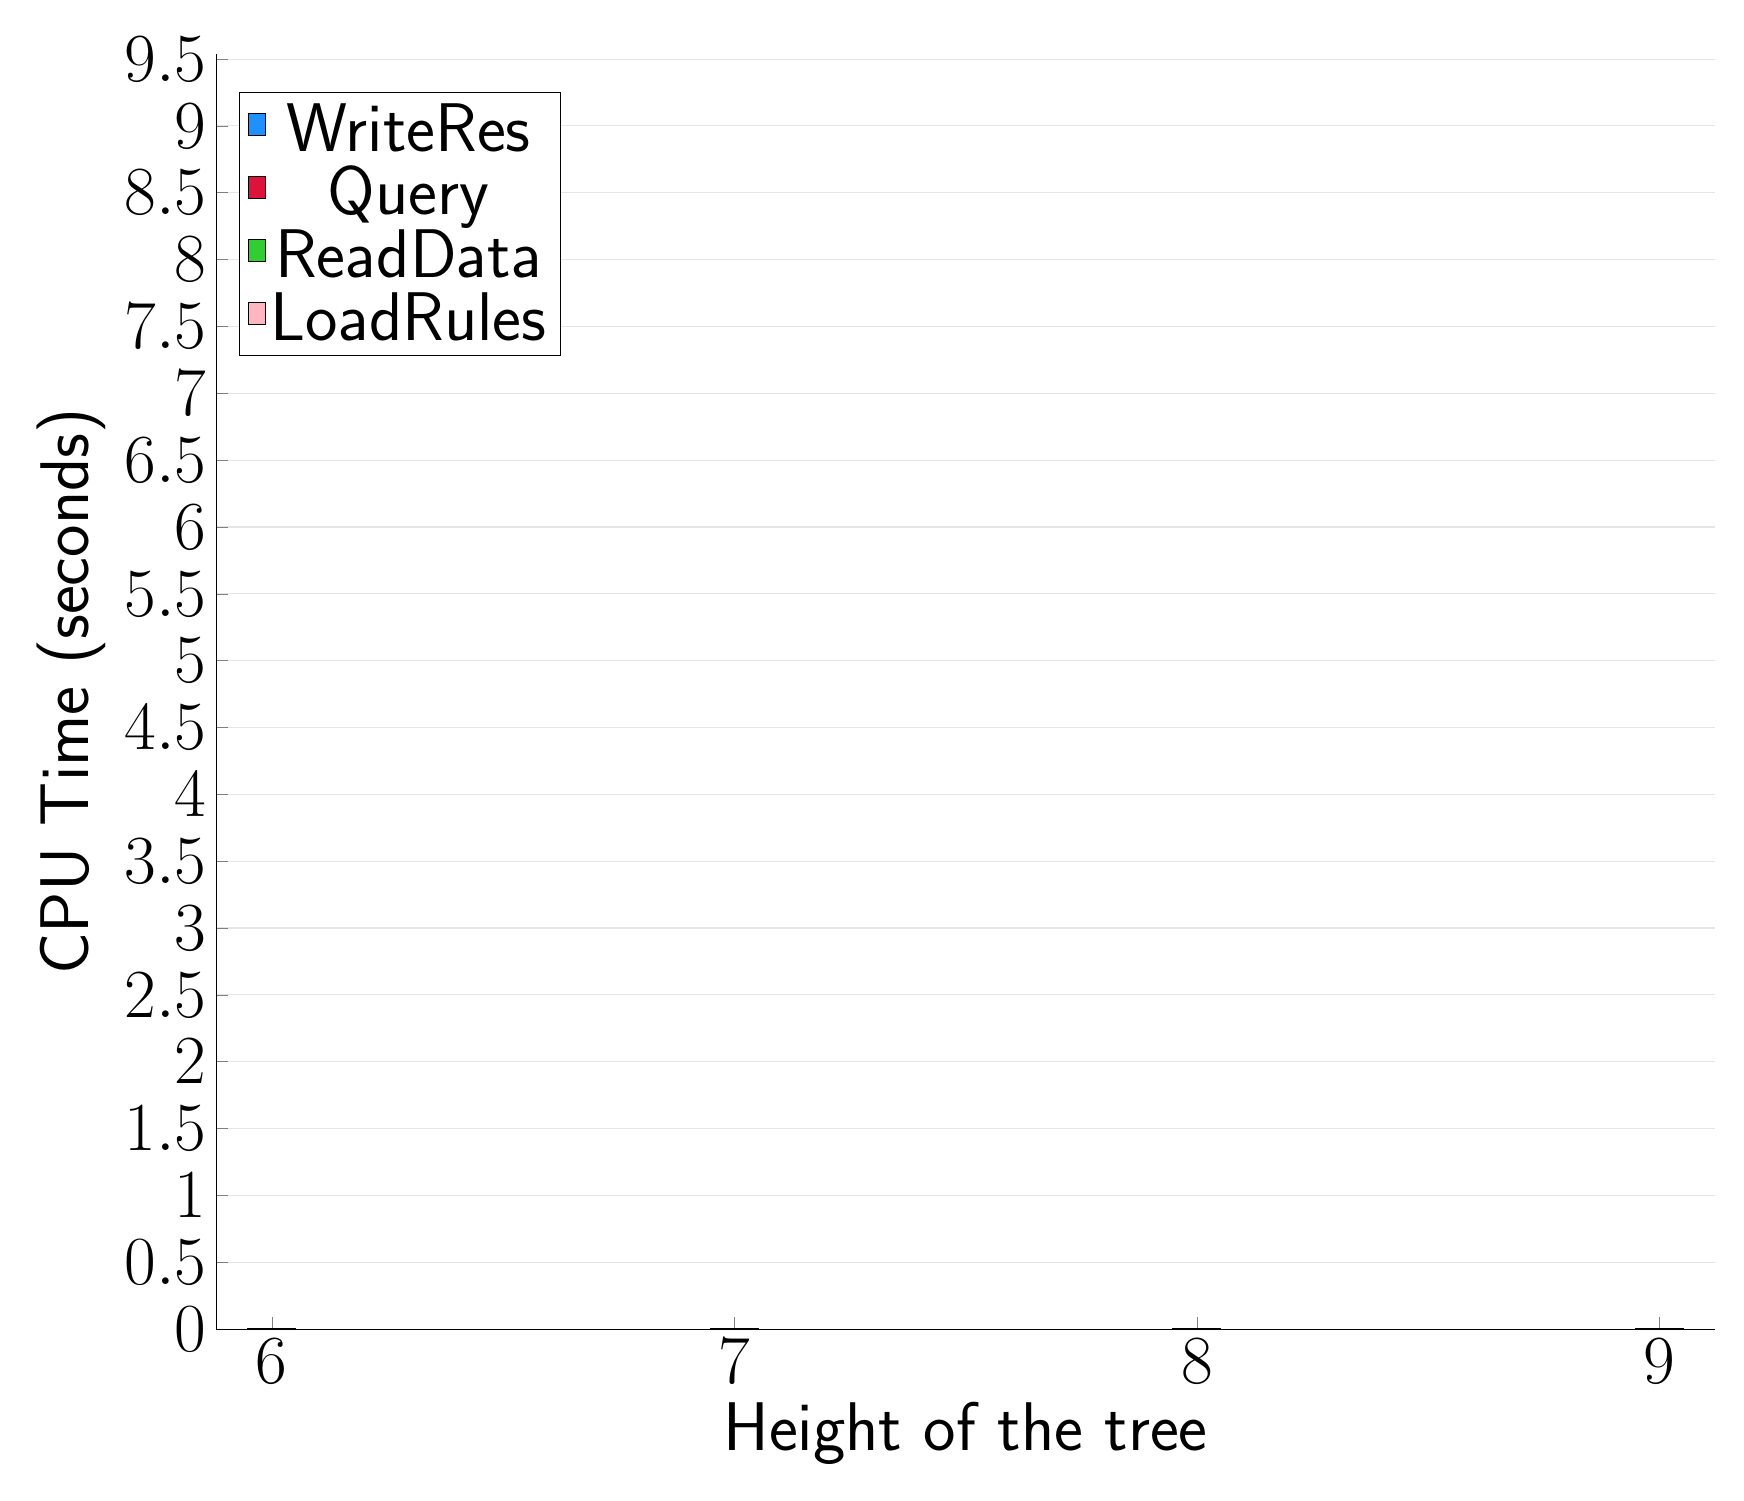
\begin{tikzpicture}
\begin{axis}[
   ybar stacked,
   width=1.7\textwidth,
   bar width=0.6cm,
   ymajorgrids, tick align=inside,
   major grid style={draw=gray!20},
   xtick=data,
   ymin=0, ymax=9.54,
   axis x line*=bottom,
   axis y line*=left,
   enlarge x limits=0.04,
   legend style={
       at={(0.23, 0.97)},
       anchor=north east,
       legend columns=1,
       font=\Huge,
   },
   ylabel={CPU Time (seconds)},
   xlabel={Height of the tree},
   label style={font=\Huge},
   tick label style={font=\Huge},
]
\addlegendimage{fill=DodgerBlue, draw=black, line width=0.2pt}
\addlegendentry{WriteRes}
\addlegendimage{fill=Crimson, draw=black, line width=0.2pt}
\addlegendentry{Query}
\addlegendimage{fill=LimeGreen, draw=black, line width=0.2pt}
\addlegendentry{ReadData}
\addlegendimage{fill=LightPink, draw=black, line width=0.2pt}
\addlegendentry{LoadRules}
\addplot +[fill=LightPink, draw=black, line width=0.55pt] coordinates {
(6, 0.0005678000000000004)
(7, 0.0005607999999999992)
(8, 0.0005537999999999999)
(8, 0.0005518000000000001)
(8, 0.0005537999999999998)
(9, 0.0005532000000000009)
(9, 0.0005554000000000004)
(9, 0.0005566000000000002)
(9, 0.0005534000000000004)
(9, 0.00055)
};
\addplot +[fill=LimeGreen, draw=black, line width=0.55pt] coordinates {
(6, 0.0001771999999999998)
(7, 0.00022540000000000044)
(8, 0.00032399999999999936)
(8, 0.00031979999999999975)
(8, 0.000327)
(9, 0.0005312)
(9, 0.0005246)
(9, 0.0005295999999999998)
(9, 0.0005279999999999999)
(9, 0.0005367999999999996)
};
\addplot +[fill=Crimson, draw=black, line width=0.55pt] coordinates {
(6, 3.1199999999999986e-05)
(7, 5.6199999999999686e-05)
(8, 0.00011160000000000019)
(8, 0.00011320000000000041)
(8, 0.00011280000000000021)
(9, 0.0002347999999999998)
(9, 0.0002335999999999996)
(9, 0.0002382000000000002)
(9, 0.0002372)
(9, 0.00023500000000000018)
};
\addplot +[fill=DodgerBlue, draw=black, line width=0.55pt] coordinates {
(6, 7.999999999999983e-05)
(7, 9.940000000000072e-05)
(8, 0.0001394000000000002)
(8, 0.00013759999999999922)
(8, 0.00014120000000000023)
(9, 0.00022480000000000018)
(9, 0.0002202000000000002)
(9, 0.00022620000000000002)
(9, 0.0002137999999999994)
(9, 0.0002169999999999994)
};
\end{axis}
\end{tikzpicture}

\end{document}
